\documentclass{scrreprt}

\usepackage{aligned-overset}
\usepackage{amsmath}
\usepackage{amssymb}
\usepackage{bm}
\usepackage[shortlabels]{enumitem}
\usepackage{hyperref}
\usepackage[utf8]{inputenc}
\usepackage{mathtools}
\usepackage{physics}
\usepackage{tabularx}
\usepackage{titling}
\usepackage{fancyhdr}
\usepackage{xfrac}
\usepackage{pgfplots}

\pgfplotsset{compat = newest}
\usepgfplotslibrary{fillbetween}

\author{}
\date{SoSe 2021}
\title{Hausaufgabe 08 \\Analysis - Weiterführende Konzepte}

\setlength{\headheight}{26pt}
\pagestyle{fancy}
\fancyhf{}
\lhead{\thetitle}
\rhead{\theauthor}
\lfoot{\thedate}
\rfoot{Seite \thepage}

\begin{document}
\paragraph{Hausaufgabe 1} Geben Sie den größtmöglichen Definitionsbereich
$D(f) \subseteq \mathbb{R}^N$ der folgenden Ausdrücke an.
Auf welcher Teilmenge $D(f') \subseteq D(f)$ existieren die Ableitungen $f'$?
Ermitteln Sie die zugehörige Jacobi-Matrix $J_f(x)$.
\begin{enumerate}[a)]
\item $f(x_1, x_2) = \ln(2 - e^{x_1 - x_2})$
  \subparagraph{Lösung:}
  $D(f) = \qty{(x_1, x_2) \in \mathbb{R}^2 {\Big |} x_1 - x_2 \leq \ln 2}$
  \begin{flalign*}
    J_f(x) &= \begin{pmatrix}
      - \frac{e^{x_1 - x_2}}{2 - e^{x_1 - x_2}} &
      \frac{e^{x_1 - x_2}}{2 - e^{x_1 - x_2}}
    \end{pmatrix} & \\
    D(f') &= \qty{(x_1, x_2) \in \mathbb{R}^2 {\Big |} x_1 - x_2 \ne \ln 2}
  \end{flalign*}

\item $f(x_1, x_2, x_3) = \qty(1 + \ln x_1, x_1\sqrt{x_2}, \sqrt{x_1x_3})$
  \subparagraph{Lösung:}
  $D(f) = \qty{(x_1, x_2, x_3) \in \mathbb{R}^3 {\Big |} x_1, x_2, x_3 \geq 0}$
  \begin{flalign*}
    J_f(x) &= \begin{pmatrix}
      \frac{1}{x_1} & 0 & 0 \\
      \sqrt{x_2} & - \frac{x_1}{\sqrt{x_2}} & 0 \\
      0 & 0 & - \frac{x_1}{\sqrt{x_1x_3}}
    \end{pmatrix} & \\
    D(f,) &= \qty{(x_1, x_2, x_3) \in \mathbb{R}^2 {\Big |} x_1 \ne 0, x_2 > 0, x_1 \cdot x_3 \geq 0}
  \end{flalign*}

\item $f(t) = e^t(\cos t, \sin t, 1)$
  \subparagraph{Lösung:} $D(f) = \qty\big{t \in \mathbb{R}}$
  \begin{flalign*}
    J_f(t) &= e^t \cdot \begin{pmatrix}
      \sin t + \cos t \\
      \cos t - \sin t \\
      1
    \end{pmatrix} & \\
    D(f') &= \qty\big{t \in \mathbb{R}}
  \end{flalign*}
\end{enumerate}

\newpage
\paragraph{Hausaufgabe 2} Gegeben sei die Funktion
$f \colon \mathbb{R}^2 \to \mathbb{R}$ mit
\begin{flalign*}
  f(x) &\coloneqq \begin{cases}
    \frac{x_1x_2}{\sqrt{x_1^2 + x_2^2}}, & \text{für } x = \qty(x_1, x_2) \ne (0, 0) \\
    0, & \text{für } x = (0, 0)
  \end{cases} &
\end{flalign*}
\begin{center}
  \resizebox{.8\textwidth}{!}{
    \begin{tikzpicture}[
        declare function={
          f(\x, \y) = \x^2 + \y^2 != 0 ? (\x*\y)/(sqrt(\x^2 + \y^2)) : 0;
        }
      ]
      \begin{axis}[
        xlabel = $x$,
        ylabel = $y$,
        view={20}{40},
      ]
        \addplot3[
          surf,
          domain=-1:1,
          samples=25,
          shader=faceted interp,
        ] {f(x, y)};
      \end{axis}
    \end{tikzpicture}
  }
\end{center}

\begin{enumerate}[a)]
\item Zeigen Sie, dass $f$ in $(0, 0)$ stetig ist.
  \subparagraph{Lösung:} Die Funktion $f$ heißt stetig im Punkt
  $x_0 = (0, 0) \in \mathbb{R}^2$, wenn
  \begin{flalign*}
    \forall \epsilon > 0 \:\exists\: \delta > 0 \forall y \in \mathbb{R}^2 \colon \norm{x_0 - y}_2 < \delta
    &\Rightarrow \abs{f(x_0) - f(y)} < \epsilon & \\
    \sqrt{y_1^2 + y_2^2} < \delta &\Rightarrow \abs{\frac{y_1y_2}{\sqrt{y_1^2 + y_2^2}}} < \epsilon \\
    \sqrt{y_1^2 + y_2^2} < \delta &\Rightarrow \frac{\abs{y_1y_2}}{\sqrt{y_1^2 + y_2^2}} < \epsilon \\
    \sqrt{y_1^2 + y_2^2} < \delta &\Rightarrow \sqrt{y_1^2 + y_2^2} \cdot \frac{\abs{y_1y_2}}{y_1^2 + y_2^2} < \epsilon \\
    \sqrt{y_1^2 + y_2^2} < \delta &\Rightarrow \sqrt{y_1^2 + y_2^2} \cdot \frac{1}{\abs{\frac{y_1}{y_2}} + \abs{\frac{y_2}{y_1}}}
    \leq \frac{\sqrt{y_1^2 + y_2^2}}{2} < \epsilon
  \end{flalign*}
  $\Rightarrow f$ ist im Punkt $(0, 0)$ stetig mit $\delta > 2\epsilon$.

\newpage
\item Zeigen Sie, dass die partiellen Ableitungen $f$ in $(0, 0)$ existieren.
  Existiert die Richtungsableitung von $f$ in $(0, 0)$ in Richtung von
  $v = \frac{1}{\sqrt{2}}\qty(e_1 + e_2) = \frac{1}{\sqrt{2}(1, 1)}$?
  Warum ist $f$ in $(0, 0)$ nicht differenzierbar?

  \subparagraph{Lösung:} Für $t \in \mathbb{R}$ gilt
  \colorbox{yellow}{$g(t) = f(t, 0) = 0 = f(0, t)$}.
  Folglich ist
  \begin{flalign*}
    \frac{\partial^nf(0,0)}{\partial x_1^n} &=
    \frac{\partial^n f(0, 0)}{\partial x_2^n} = g^{(n)}(0) = 0
    \text{ für alle } n \in \mathbb{N}
  \end{flalign*}

  Die Funktion $f$ heißt in $x = (0, 0) \in \mathbb{R}^2$ in Richtung
  $v = \frac{1}{\sqrt{2}(1, 1)}$ differenzierbar, falls die Funktion
  \[
    k \colon ]-r, r[ \to \mathbb{R}, t \mapsto f(x + t \cdot v)
  \]
  (für $r > 0$ klein genug) in $0$ differenzierbar ist und dann heißt
  \[
    \frac{\partial f}{\partial v}(x) \coloneqq \lim_{t \to 0} \frac{k(t) - f(x)}{t}
  \]
  die Richtungsableitung von $f$ im Punkt $(0, 0)$ in Richtung $v$.

  \[
    k(t) = f((0,0) + t \cdot v) = f\qty(\frac{t}{\sqrt(2)}, \frac{t}{\sqrt(2)})
    = \begin{cases}
      \frac{\sfrac{t^2}{2}}{\sqrt{2\sfrac{t^2}{2}}} = \frac{t}{2} & t \ne 0 \\
      0 & t = 0
    \end{cases}
  \]
  Da für $t = 0$ der Wert von $\frac{t}{2} = k(0)$ entspricht, gilt
  $k(t) = \frac{t}{2}$.
  $\Rightarrow$ die Richtungsableitung von $f$ im Punkt $(0, 0)$ in Richtung
  $v$ existiert mit
  \[
    \frac{\partial f}{\partial v}(x) \coloneqq \lim_{t \to 0} \frac{k(t) - f(x)}{t}
    = \lim_{t \to 0} \frac{\sfrac{t}{2} - f((0,0))}{t} = \frac{1}{2}
  \]

  Die \colorbox{yellow}{partiellen Ableitungen} entsprechen den
  Richtungsableitungen $u_1 = e_1$ und $u_2 = e_2$.
  Da
  $\frac{\partial f}{\partial u_1}(x) = 0 \ne \frac{\partial f}{\partial v}(x) = \frac{1}{2}$
  ist $f$ im Punkt $(0, 0)$ nicht differenzierbar.


\end{enumerate}

\newpage
\paragraph{Hausaufgabe 3} Gegeben seien die Funktionen
$f \colon (0, \infty) \times (0, \infty) \to \mathbb{R}^2$ und
$g \colon \mathbb{R}^2 \setminus \qty{(0, 0)} \to \mathbb{R}$ mit
$f(x, y) \coloneqq \qty(xy, \frac{\sqrt{x}}{y})$ und
$g(u, v) \coloneqq \ln\qty(u^2 + v^2)$.
Berechnen Sie die Jacobi-Matrix der verketteten Funktion
$\ell = g \circ f \colon (0, \infty) \times (0, \infty) \to \mathbb{R}^2$
auf direktem Weg und durch Anwendung der Kettenregel.

\subparagraph{Lösung:} $\ell(x, y) = (g \circ f)(x, y) = g\qty\big(f(x , y))$

\textbf{Direkter Weg:} $\ell (x, y) = g\qty(x \cdot y, \frac{\sqrt{x}}{y}) = \ln\qty(x^2y^2 + \frac{x}{y^2})$

\begin{flalign*}
  J_{\ell}(x, y) &= \begin{pmatrix}
    \frac{2xy^2 + \frac{1}{y^2}}{x^2y^2 + \frac{x}{y^2}} &
    \frac{2x^2y - \frac{2x}{y^3}}{x^2y^2 + \frac{x}{y^2}}
  \end{pmatrix} =
  \begin{pmatrix}
    \frac{2xy^4 + 1}{x^2y^4 + x} &
    \frac{2xy^4 - 2}{xy^5 + y}
  \end{pmatrix}&
\end{flalign*}

\textbf{Kettenregel:} $J_f = \begin{pmatrix}
  y & x \\
  \frac{1}{2y\sqrt{x}} & -\frac{\sqrt{x}}{y^2}
\end{pmatrix}$ und
$J_g = \begin{pmatrix}
  \frac{2u}{u^2 + v^2} & \frac{2v}{u^2 + v^2}
\end{pmatrix}$
\begin{flalign*}
  J_{\ell}
  &= J_g(f(x, y)) \cdot J_f(x, y)
  = J_g\qty(xy, \frac{\sqrt{x}}{y}) \cdot J_f(x, y) & \\
  &= \begin{pmatrix}
    \frac{2xy}{x^2y^2 + \frac{x}{y^2}} & \frac{\frac{2\sqrt{x}}{y}}{x^2y^2 + \frac{x}{y^2}}
  \end{pmatrix} \cdot
  \begin{pmatrix}
    y & x \\
    \frac{1}{2y\sqrt{x}} & -\frac{\sqrt{x}}{y^2}
  \end{pmatrix} \\
  &= \begin{pmatrix}
    \frac{2xy}{x^2y^2 + \frac{x}{y^2}} \cdot y + \frac{\frac{2\sqrt{x}}{y}}{x^2y^2 + \frac{x}{y^2}} \cdot  \frac{1}{2y\sqrt{x}} &
    \frac{2xy}{x^2y^2 + \frac{x}{y^2}} \cdot x + \frac{\frac{2\sqrt{x}}{y}}{x^2y^2 + \frac{x}{y^2}} \cdot  -\frac{\sqrt{x}}{y^2}
  \end{pmatrix} \\
  &= \begin{pmatrix}
    \frac{2xy^2 + \frac{1}{y^2}}{x^2y^2 + \frac{x}{y^2}} &
    \frac{2x^2y - \frac{2x}{y^3}}{x^2y^2 + \frac{x}{y^2}}
  \end{pmatrix} =
  \begin{pmatrix}
    \frac{2xy^4 + 1}{x^2y^4 + x} &
    \frac{2xy^4 - 2}{xy^5 + y}
  \end{pmatrix}
\end{flalign*}

\end{document}